\begin{figure}[ht]
  \captionsetup[subfloat]{labelformat=empty}

  \begin{tabular}{ccccc}

    \subfloat[\texttt{Insert(40)}]{
      \begin{tikzpicture}
        \node [circle] (z){$40$}
        child[missing] {}
        child[missing] {};
      \end{tikzpicture}
    } &

    \subfloat[fix II.]{
      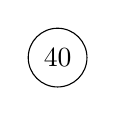
\begin{tikzpicture}
        \node [circle,draw] (z){$40$}
        child[missing] {}
        child[missing] {};
      \end{tikzpicture}
    } &

    \subfloat[\texttt{Insert(48)}]{
      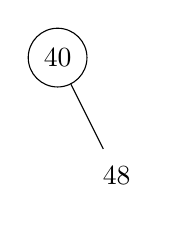
\begin{tikzpicture}
        \node [circle,draw] (z){$40$}
        child[missing] {}
        child {
            node [circle] (a) {48}
            child[missing] {}
            child[missing] {}
          };
      \end{tikzpicture}
    } &

    \subfloat[\texttt{Insert(68)}]{
      \begin{tikzpicture}
        \node [circle,draw] (z){$40$}
        child[missing] {}
        child {
            node [circle] (a) {48}
            child[missing] {}
            child {
                node [circle] (b) {68}
                child[missing] {}
                child[missing] {}
              }
          };
      \end{tikzpicture}
    } &

    \subfloat[fix IV.6]{
      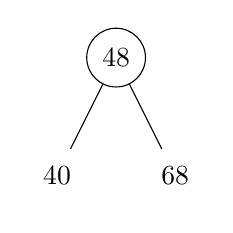
\begin{tikzpicture}
        \node [circle,draw] (z){$48$}
        child {
            node [circle] (a) {40}
            child[missing] {}
            child[missing] {}
          }
        child {
            node [circle] (b) {68}
            child[missing] {}
            child[missing] {}
          };
      \end{tikzpicture}
    }   \\

    \subfloat[\texttt{Insert(55)}]{
      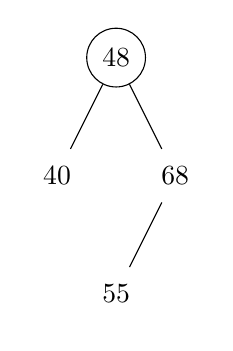
\begin{tikzpicture}
        \node [circle,draw] (z){$48$}
        child {
            node [circle] (a) {40}
            child[missing] {}
            child[missing] {}
          }
        child {
            node [circle] (b) {68}
            child {
                node [circle] (c) {55}
                child[missing] {}
                child[missing] {}
              }
            child[missing] {}
          };
      \end{tikzpicture}
    } &

    \subfloat[fix IV.4]{
      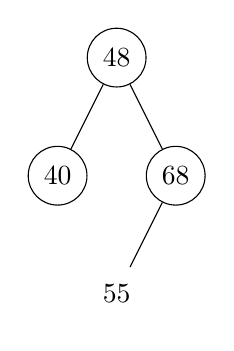
\begin{tikzpicture}
        \node [circle,draw] (z){$48$}
        child {
            node [circle,draw] (a) {40}
            child[missing] {}
            child[missing] {}
          }
        child {
            node [circle,draw] (b) {68}
            child {
                node [circle] (c) {55}
                child[missing] {}
                child[missing] {}
              }
            child[missing] {}
          };
      \end{tikzpicture}
    } &

    \subfloat[\texttt{Insert(39)}]{
      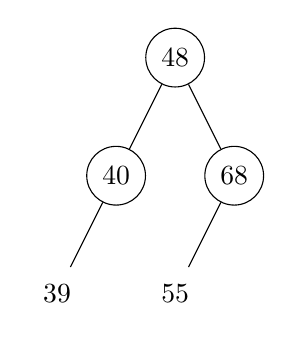
\begin{tikzpicture}
        \node [circle,draw] (z){$48$}
        child {
            node [circle,draw] (a) {40}
            child {
                node [circle] (c) {39}
                child[missing] {}
                child[missing] {}
              }
            child[missing] {}
          }
        child {
            node [circle,draw] (b) {68}
            child {
                node [circle] (d) {55}
                child[missing] {}
                child[missing] {}
              }
            child[missing] {}
          };
      \end{tikzpicture}
    } &

    \subfloat[\texttt{Delete(40)}]{
      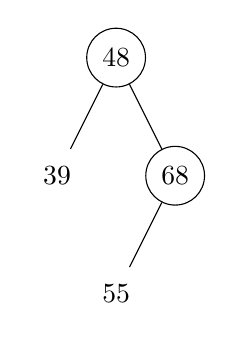
\begin{tikzpicture}
        \node [circle,draw] (z){$48$}
        child {
            node [circle] (a) {39}
            child[missing] {}
            child[missing] {}
          }
        child {
            node [circle,draw] (b) {68}
            child {
                node [circle] (d) {55}
                child[missing] {}
                child[missing] {}
              }
            child[missing] {}
          };
      \end{tikzpicture}
    } &

    \subfloat[fix IV.3]{
      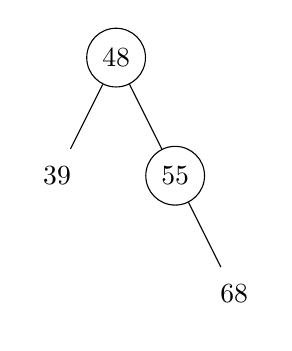
\begin{tikzpicture}
        \node [circle,draw] (z){$48$}
        child {
            node [circle] (a) {39}
            child[missing] {}
            child[missing] {}
          }
        child {
            node [circle,draw] (b) {55}
            child[missing] {}
            child {
                node [circle] (c) {68}
                child[missing] {}
                child[missing] {}
              }
          };
      \end{tikzpicture}
    }   \\

    \subfloat[fix IV.4]{
      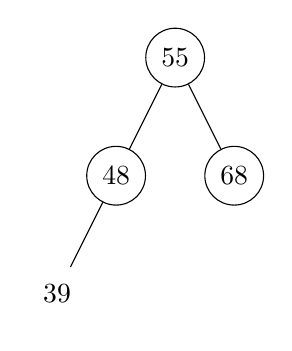
\begin{tikzpicture}
        \node [circle,draw] (z){$55$}
        child {
            node [circle,draw] (a) {48}
            child {
                node [circle] (b) {39}
                child[missing] {}
                child[missing] {}
              }
            child[missing] {}
          }
        child {
            node [circle,draw] (c) {68}
            child[missing] {}
            child[missing] {}
          };
      \end{tikzpicture}
    } &

    \subfloat[\texttt{Delete(48)}]{
      \centering
      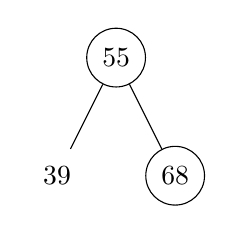
\begin{tikzpicture}
        \node [circle,draw] (z){$55$}
        child {
            node [circle] (a) {39}
            child[missing] {}
            child[missing] {}
          }
        child {
            node [circle,draw] (b) {68}
            child[missing] {}
            child[missing] {}
          };
      \end{tikzpicture}
    } &

    \subfloat[fix IV.2]{
      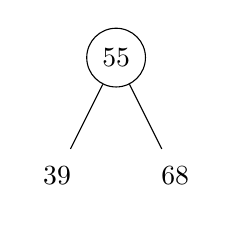
\begin{tikzpicture}
        \node [circle,draw] (z){$55$}
        child {
            node [circle] (a) {39}
            child[missing] {}
            child[missing] {}
          }
        child {
            node [circle] (b) {68}
            child[missing] {}
            child[missing] {}
          };
      \end{tikzpicture}
    }
  \end{tabular}

  \caption{Rot-Schwarz-Baum nach Einfüge- und Löschoperationen}\label{fig:rbinsdel}
\end{figure}